\chapter{Strongly coupled PAS of a weakly bound molecule} \label{ch:chap4}
\section{Probing the ground state potential} \label{sec:highE_intro}
Weakly bound ground-state dimers are of great interest in ultracold atomic and molecular physics. 
In this chapter we study the least-bound vibrational level of the X$^1\Sigma_g^+$ electronic ground state of the $^{86}$Sr$_2$ dimer in a high intensity regime, where the AC Stark shift is comparable to the unperturbed binding energy.

Previous studies of the molecular states of the X$^1\Sigma_g^+$ ground state potential have primarily focused on strontium-88.
Lots of properties of strontium derived from these studies and applied to other isotopes via mass-scaling.
This work presents the first two-photon photoassociation study of the ground state of $^{86}$Sr, as all previous PA experiments have been one-photon PA to excited electronic states \hl{Yu 25-27}.
Direct excitation to the halo state provides an extremely sensitive probe of the long-range part of the ground state potential.
The work presented in this chapter was followed by a low intensity study, presented in Ch.\,\ref{ch:chap5}, which precisely determined the natural halo binding energy and presents a mass-scaled theory improving on the accepted scattering lengths of all strontium isotopes.

In these initial experiments, when varying the excitation laser intensity, we observed unexpectedly large bound-bound coupling between the intermediate molecular state, used for Raman coupling, and the halo state.
Furthermore, by varying the intermediate state detuning, we observed a breakdown of the isolated resonance model which cannot explain the observed frequency dependence of the AC stark shift of the two-photon transition.

As discussed in the previous chapter, two-photon PAS can be used to directly populate molecular levels and can be described using the theory of Bohn and Julienne if the two driving lasers are of sufficently different frequencies such that each laser independently drives a specific transition.
This corresponds to the typical $\Lambda$-model \hl{Yu, 20 21}.
However, in the scenario of the halo state, the laser frequencies differ by only up to $\sim$300\,kHz which is much smaller than the typical intermediate state detuning of several MHz.
In this regime, each laser should be considered to act on both legs of the transition leading and in collaboration with the theory group of Kaden Hazzard, we developed simple theoretical models for describing this novel regime.

In the following we present our high-intensity results and discuss the theoretical development of several models focused on predicting the observed frequency dependence of the halo state and the bound-bound coupling to the intermediate state.

\section{Experimental setup} \label{sec:highE_methods}
Fig.\,\ref{fig:PASDiagram} shows the excitation scheme used to probe the halo state in $^{86}$Sr using two-photon Raman photoassociation \cite{jtl06}, in which two laser fields couple colliding atoms to the least-bound state of the ground molecular potential. 
	\begin{figure} 
	\centerline{
	  \includegraphics[width=\textwidth]{sr_pa_potential.pdf}}
	  \caption{Strontium PAS potential}{Two-photon photoassociation diagram. The energy of two well-separated $^1S_0$ atoms at rest is taken as zero. $\epsilon$ is the kinetic energy of the colliding atom pair. $E_{b1}$ is the unperturbed energy of the bound state of the excited molecular potential that is near resonance with the free-bound laser, which in these experiments is the second-least bound level of the excited molecular potential ($\nu=-2$). $E_{b2}$ ($<0$) is the unperturbed energy of the least bound state of the ground molecular potential. The photon of energy $\hbar \omega_1$ is detuned from $E_{b1}$ by $\hbar \Delta_1$ for $\epsilon=0$, while the two-photon detuning from $E_{b2}$ is $\hbar \Delta_2$. The decay rate of $b_1$ is $\gamma_1$. Stark and collisional frequency shifts are neglected in this schematic.}
	  \label{fig:PASDiagram}
	\end{figure}
The sample temperature is low enough that collisions are entirely $s$-wave. 
The target state for the two-photon transition has total angular momentum $J=0$ and binding energy $E_{b2}(<0)$. $^{86}$Sr has no nuclear spin and a $^1S_0$ electronic ground state, leading to a single ground electronic molecular potential (X$^1\Sigma_g^+$). 
The dominant intermediate state ($b_1$) is the $J=1$ rotational state of the second least-bound ($\nu=-2$) vibrational level on the $0^+_u$ molecular potential, which asymptotically connects to the $^1S_0+ {^3P_1}$ asymptote at long range\cite{mmp08}.
This state is bound by $44.246(10)$\,MHz \cite{bmc14}.
We define $\Delta_1=\omega_1-E_{b1}/\hbar$ and $\Delta_2=\omega_1-\omega_2-E_{b2}/\hbar$ as the one-photon detuning from state $b_1$ and two-photon detuning from state $b_2$ respectively for an initial scattering state with collision energy $\epsilon=0$.
$\Omega_{2,12}$ is the Rabi frequency for coupling between states $b_1$ and $b_2$ due to the laser field at $\omega_2$ with single-beam intensity $I_2$.
Because the binding energy of the halo molecule is very small compared to $\Delta_1$, both laser frequencies are near resonance with the $\nu=-2$ state. 
The transitions to the least-bound ($\nu=-1$) $J=1$ excited molecular state, bound by $1.633(1)$\,MHz, and the excited atomic state lie near enough in energy that they can effect our observations.	

Photoassociation leads to loss of atoms from the trap through radiative decay from the intermediate, excited electronic state, and from collisions between molecules and background atoms.
In addition to the relevant potentials, Fig.\,\ref{fig:PASDiagram} also defines two possible relationships  between the laser frequencies.
In each of these scenarios, the frequency of $\omega_1$ remains fixed while the frequency of $\omega_2$ is varied.
In the case that $\omega_2 > \omega_1$, then the standard Raman configuration is recovered where $\Delta_1$ remains fixed while increasingly more energy is withdrawn from the system as $\omega_2$ is increased.
In the opposing scenario, $\omega_2 < \omega_1$, $\Delta_1$ is also varied slightly as $\omega_2$ is varied, which in turn leads to a changing AC Stark shift over the course of a scan.
Although, in our experiments $\Delta_2 \ll \Delta_1$ and subsequently the variation of the AC Stark shift acting on the halo state is small.
While experimentally, the data presented in this chapter is not accurate enough to measure the effects of this variation, our theoretical model does predict slightly different binding energies in these two regimes as discussed below.
 
After an exposure time on the order of one hundred milliseconds, the number of ground-state atoms remaining and the sample temperature are measured with time-of-flight absorption imaging.

%% Sample properties and trap description
Two-photon spectroscopy is performed on ultracold $^{86}$Sr atoms in a single-beam optical dipole trap generated from a 1064-nm laser propagating perpendicular to gravity with beam waists of 260 and 26\,$\mu$m [17,22].
The tight waist provides vertical confinement.
The trap depth after an evaporative cooling stage determines the sample temperature, which is set between 30 and 1000 nK.
Typical atom numbers are several hundred thousand and peak densities are as high as \peakDens{2}{12}.
The number of atoms and sample temperature are measured using time-of-flight absorption imaging operating on the 1S0-1P1 transition.
Trap oscillation frequencies are determined by measuring dipole and breathing collective mode frequencies, which allow determination of trap volume and sample density

 performed on ultracold Sr atoms in a single-beam optical dipole trap (ODT) generated from a 1064-nm laser propagating perpendicular to gravity.
 Typical atom numbers are several hundred thousand and peak densities are $\approx \peakDens{1}{12}$.
 The number of atoms and sample temperature are measured using time-of-flight absorption imaging described in \hl{some section}.
 Trap oscillation frequencies are determined by measuring dipole and breathing collective mode frequencies, which allow determination of trap volume and sample density
 
 
%% PAS light generations
We generate the two photons for spectroscopy as shown in Fig\ref{fig:pas_light_gen}.
	\begin{figure} \label{fig:pas_light_gen}
		\centerline{
		\includegraphics[height=0.25\textheight]{pa_exp_setup.pdf}}
		\caption{Schematic of PAS light generation}{Light for these experiments is generated by the spectroscopy slave laser setup discussed in Sec.\,\ref{sec:specSlave}.}
	\end{figure} 
These photons are injection locked from the master laser and precisely controlled via two RF frequencies incident on a single acouto-optic modulator and delivered to the atoms with an optical fiber.
This fiber output is launched near the science chamber with output optics that yield a 320\,$\mu$m waist at the atoms, much larger than the size of the atom cloud.
Both PA beams are linearly polarized along the same direction.
The beat signal of the two light fields after the fiber is monitored on a photodiode and the RF powers are adjusted to ensure matched intensities for the two frequency components ($I_1=I_2\equiv I$).


The optical fiber ensures that the wavevector of the two photons will be parallel which allows us to neglect any effects of Doppler broadening which might result from imparting momentum into the atomic sample.
 
This is a simple system for generating multiple frequencies which are gauranteed to share the same wavevector, phase coherence, and gross frequency stability. 

Primary reasons why we can't scan large distances. 
There will be a slight misalignment of the beams into the fiber and the RF may start to fall off. 
For these experiments an AOM with a center frequecny of 90 MHz was used. 

We see a reduction in contrast when the two drive frequencies differ by more than $\approx$250 kHz. 

Since the modulator is a narrowband device, scann

great care is taken to ensure the maximum amount of contrast is visible on the photodiode. This 




This simple system has many advantages and a couple of drawbacks. 
Since both photons are aligned into the same fiber then they are gauranteed to have the same output wavevector and therefore the two photon process will be doppler free (since the absorption and emission processes will exactly cancel each other out).


Use of the AOM provides highly accurate control of the difference frequency with RF precision. 

While versatile and simple, we are worried about the balnace of the RF power onto the AOM. THese devices are narrowband modulators (simple ones) 



As described in \hl{some section} the slave laser is frequency stabiliezed at +42 MHz of the 86Sr $\gs\,\rightarrow\,\ex$ atomic transition. The AOM then shifts the light the remaining $\approx$ 86 MHz to set the detuning around the $\nu=-2$ bound state of the \intPot{\gs}{\ex} potential. 
Setting of $\Delta_1$ is done by removing one of the frequencies, peaking up the diffraction angle and alignment into the fiber. 

During the course of our experiments we found that mild environmental perturbations (loud noises, air currents due to fans, etc.) to the fiber resulted in slow variation of the light coupling through the fiber.
Such amplitude modulations are not uncommon in laser systems and can typically be compensated for by using a closed loop locking mechanism. 
However, after construction of such a power lock the compoenets did not react quickly enough and there was a significant overshoot which resulted in an uncontrolled amount of light illuminating the atoms during short exposures. 
This led us to implement a digital based sample and hold mechanism for reduced intensity variability. This system is described in detail in \hl{some section}. 
The sample and hold system in combination with the power lock provided intensity stability with a standard 5\% standard deviation during a typical experiment. 
Fig shows a typical histogram of the recorded intensities. 


\begin{figure} \label{fig:ch3_pas_histogram}
	\centerline{
	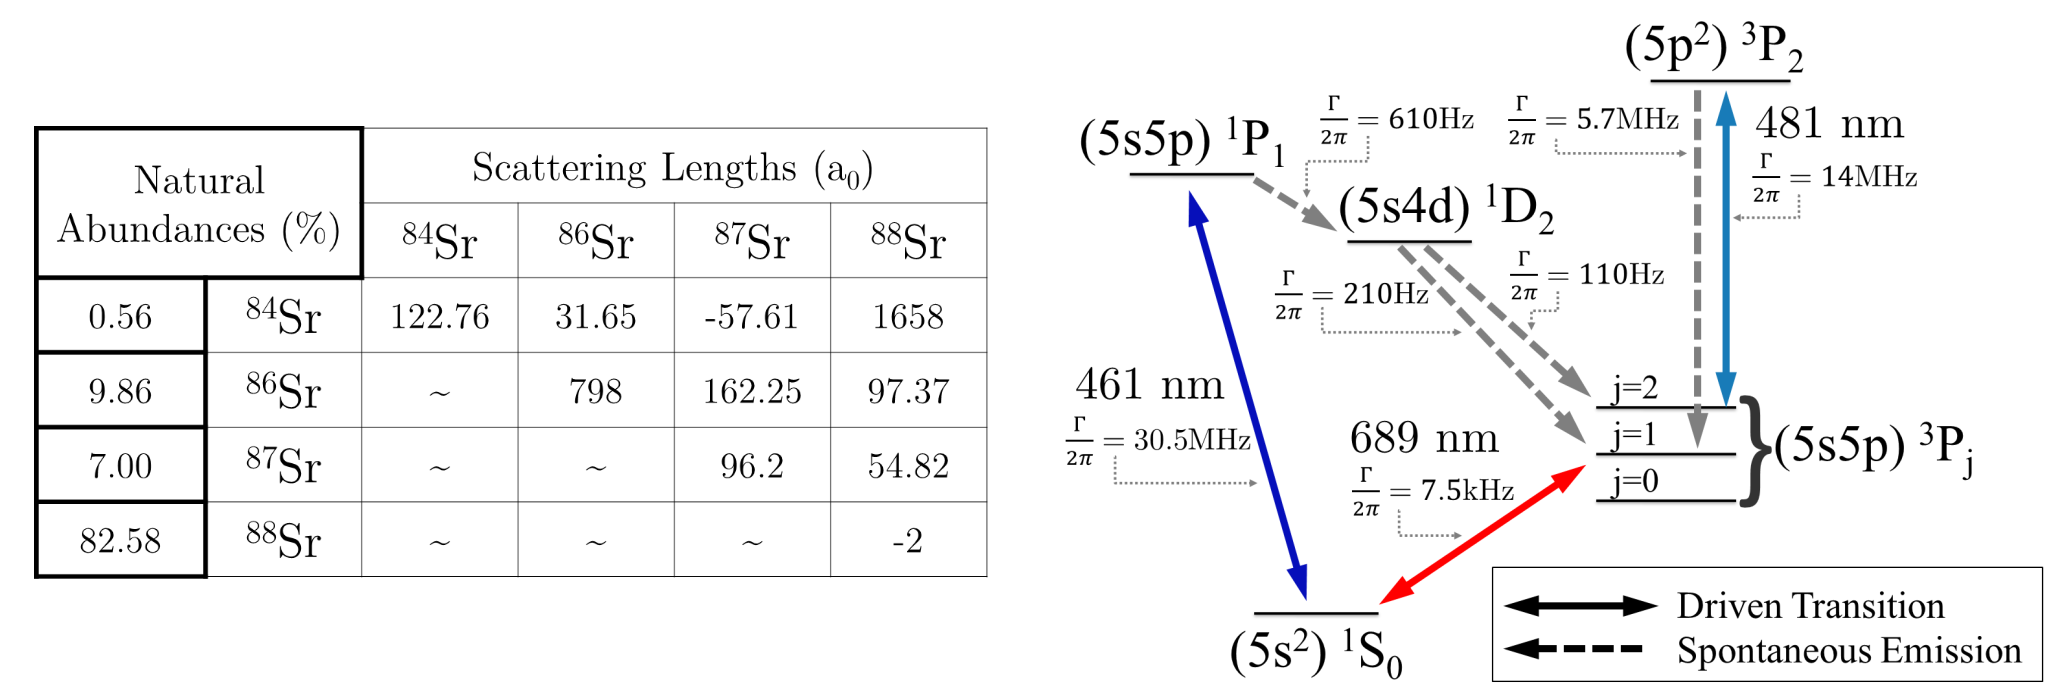
\includegraphics[height=0.25\textheight]{strontium_properties.pdf}}
	\caption{Histogram of PAS beam intensity variation}{One of the histograms from onenote. There are separate histograms for each experimental run (I should combine this so I don't have to disucss)}
\end{figure} 

The beat signal of the two light fields after the fiber is monitored on a photodiode and the rf powers are adjusted to ensure matched intensities for the two frequency components ($I_1 = I_2 \equiv I$).

\begin{figure} \label{fig:ch3_pas_light_balance}
	\centerline{
	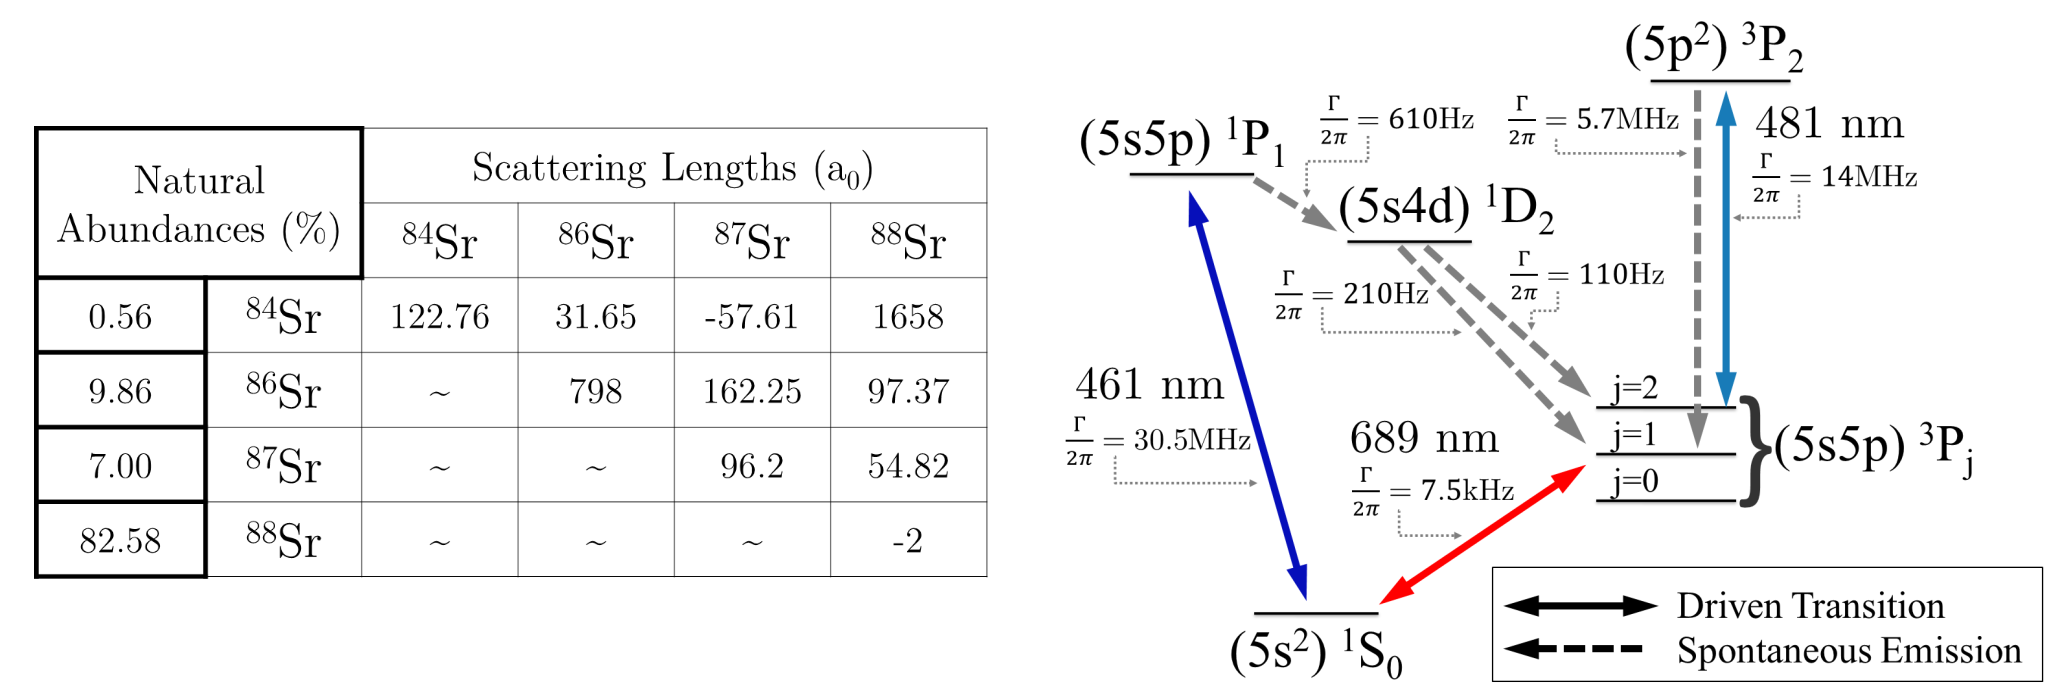
\includegraphics[height=0.25\textheight]{strontium_properties.pdf}}
	\caption{Characteristic view of the PA beatnote}{This is the picoscope plot of the beatnote}
\end{figure} 

Regarding the general process 

Using the \intPot{\gs}{\ex} interatomic potential, we perform a raman process using the $\nu=-2$ bound state which has a binding energy of E$_b=-44 \text{MHz}$ \hl{cite improved binding en}. Sample pre 

We used strontium 86 in a thermal gas at temperatures between 30 and 1000 nK. Typical peak densitieis were around $\peakDens{1}{12}$. 

Raman process using the second bound state of the \intPot{\gs}{\ex} interatomic potential

After the atoms have equilibrated in the final ODT configuration, the PA lasers are applied (Fig.\ \ref{PASDiagram}). A single acousto-optic modulator, driven with two RF frequencies, is used to generate both PA beams. Light is derived from a frequency-stablized master laser (Fig.\ \ref{Experimental Setup}) and coupled into a single-mode optical fiber 

%$I_{689}$ is varied to obtain the intensity-dependence of the two-photon transition.

%(One could in principle vary the power of both light fields independently and measure how the two-photon line position changes. This will allow us to decouple the contributing factors to the AC Stark shift. If we are going to develop a theory of the multiphoton line, it will have to be able to treat this regime as well. )


\section{Estimating the halo binding energy} \label{sec:highE_theory}

In this paper, we measure spectra in the high-intensity
regime and develop a theory that accounts for the effects of the two-frequency drive when molecular binding energy is small and excitation laser intensity is high.
The model neglects motional degrees of freedom for the
initial state of two free atoms and considers only three
levels a dimer in the ground electronic state, the intermediate dimer state in the excited electronic potential,
and two well-separated atoms. We numerically solve this model and analyze many of its features with analytic approximations. We also briefly consider extensions of this
three-level model that add extra levels to capture some
fine details of the ac Stark shift at large detuning.
We show that the three-level model captures key
experimentally observed features despite its simplicity.
Numerical simulations show that it accurately predicts
the appearance of additional spectral lines in the highintensity regime, and that these correspond to higher order non-linear processes. It accurately captures the location of the spectral peaks, including ac Stark shifts
from both lasers when intermediate state detuning, $\Delta_1$1,
is comparable to E0
b
. Furthermore, when the intensity of
the lasers is not too small, the spectral lineshapes of individual lines are reasonably well-captured. This indicates
that effects missing from this theory – the motion of the
atoms [21], interaction shifts due to molecules and atoms
scattering off of other molecules and atoms [22], and the
varying density within the trap [18] – are less relevant in
the regime of interest here.

%The observed PA spectrum is relatively simple because the
%bosonic isotopes of strontium lack hyperfine structure. As shown in
%Fig.\ \ref{PASDiagram}, ground state $^1S_0$ atoms collide on a
%single $^1\Sigma^+_g$ potential. Four molecular potentials converge
%to the $^1S_0$ + $^3P_1$ asymptote \cite{mjs01}, but only states of
%the $0^+_u$ and $1_u$ potentials are optically connected to the
%$^1\Sigma^+_g$ potential \cite{zbl06}. At the low temperatures of
%these experiments, only $s$-wave collisions occur so only $J=1$
%intermediate levels and $J=0$ and 2 final states can be populated.



%\section{Details of the Model of the Photoassociation Lineshape}
%\label{sectionappendix}



%The effective volumes used throughout this analysis are defined by
%\begin{equation}\label{eq:effectivevolumes}
%	V_{\text{q}}=\int_{\mathrm{V}} d^3r \, e^{-\frac{qU(\mathbf{r})}{k_{B}T}},
%\end{equation}
%for trapping potential $U(\mathbf{r})$.

%The collision event rate constant can be expressed as a thermal average of the scattering probability for loss, $\vert S(\epsilon,\omega_1,\omega_2,...,\mathbf{r})\vert^2$, over the collision energy $\epsilon$. 

%We also average over the trap volume to allow for the possibility that the scattering probability can vary with position in the trap due to inhomogeneity of laser intensity profiles and the density distribution [Eq.~(\ref{equationKeffective})].



%Bohn and Julienne \cite{bju96} provide an expression for $\vert S(\epsilon,\omega_1,\omega_2,...)\vert^2$ for a collision on the open channel of two ground state atoms (g) with total energy $\epsilon$ leading to loss-producing decay from the excited state $b_1$ with rate $\gamma_1$. (See Fig.\ \ref{PASDiagram}.) It yields
%\begin{eqnarray}\label{equationSprob}
%  \vert S\vert^2 =   \hspace{2.5in}&&\\
%  {(\Delta_2+\epsilon/\hbar)^2{\gamma}_1{\gamma}_s \over
%  	\left[(\Delta_1+\epsilon/\hbar)(\Delta_2+\epsilon/\hbar)-\frac{\Omega_{12}^{2}}{4}\right]^2+\left[ \frac{\gamma_1+\gamma_s}{2}\right]^2(\Delta_2+		 	\epsilon/\hbar)^2}, &&\nonumber
%\end{eqnarray}
%where all quantities are defined in the main text. For simplicity, we have omitted the light shift of $b_1$ due to coupling to the scattering continuum \cite{bju99}. Equation (\ref{equationSprob}) neglects all light shifts due to the trapping laser. Light shifts due to the photoassociation lasers coupling to states outside our model (Fig.\ \ref{PASDiagram}) are also neglected. The thermal energy is much greater than the zero-point energy for trap motion, $T\gg h\nu_{\text{trap}}/k_B$, so confinement effects are negligible \cite{zbl06}.




%For the experiments reported here, we maintain significant intermediate-state detuning, $|\Delta_1|\gg |\Omega_{12}|$. Thus we are in a Raman configuration, and near two-photon resonance the expression for the scattering probability for a given initial scattering energy Eq.~(\ref{equationSprob}) can be approximated as a Lorentzian
%\begin{eqnarray}\label{equationSprobLorentzian}
% \vert S\vert^2 \approx {A(\epsilon) \over
% \left(\Delta_2+\epsilon/\hbar-\frac{\Omega_{12}^{2}}{4(\Delta_1+\epsilon/\hbar)}\right)^2+\left[ {\Gamma_L(\epsilon)}/{2}\right]^2},
%\end{eqnarray}
%where $A$ and $\Gamma_L$ are defined in Eqs.\ (\ref{ApproxLorentzianQuantitiesMain}) and (\ref{ApproxLorentzianQuantities-2Main}).
%
%As discussed in the text, we analyze loss spectra using the effective expression, Eq.\ (\ref{equationApproxLorentzian}) to account for possible deviations from the single-channel theory \cite{bju96}.

\subsection{Frequency dependence of the AC Stark shift} \label{sec:numTheory}
%% paper
The proximity of $^{86}$Sr to a scattering resonance and the susceptibility of the halo binding energy to the intensity of the excitation light suggests  using light to tune the binding energy and scattering length as was done with optically assisted magnetic Feshbach resonances \cite{blv09,chx15}, which is closely related to the use of optical Feshbach resonances \cite{Fedichev1996a,Theis2004,Yamazaki2010,Blatt,Yan2013c}. Understanding the frequency-dependence of $\chi_{689}$ is important for investigating this possibility, so we extracted this parameter from spectra at a wide range of 689-nm laser intensities and detuning from the intermediate resonance ($\Delta_1$).

Figure \ref{Fig:ShiftsofLinesWithIntensity} shows
the resulting resonance positions, $E'_{b2}$, versus twice the single-beam intensity, $2I=I_{689}$. The shift in molecular binding energy is linear with intensity over the explored range, but varies greatly in magnitude and sign. From linear fits, we extract the AC Stark shift parameter $\chi_{689}(\Delta_1)$ through $E'_{b2}\equiv E_{b2}+h\chi_{689}(\Delta_{1}) I_{689}$ (Fig.\ \ref{Fig:ACStark}).

In the experiment, the total 689-nm intensity oscillates with 100\% contrast according to $I_{\text{total}}=I_1+I_2+2\sqrt{I_1I_2}\cos \left[(\omega_1-\omega_2)t \right]=2I\left\{1+\cos \left[(\omega_1-\omega_2)t \right]\right\}$. The functional form we use to fit the AC Stark shift reflects the time average of the intensity and neglects the interference term. To confirm that this is the correct description, we numerically solved the time-evolution for a three-level system with similar optical couplings and oscillating optical intensity as present during two-photon PA of a halo state. The Hamiltonian is
\begin{eqnarray}
H=
\left(
    \begin{array}{ccc}
      0 & \Omega_{01}\left[\mathrm{cos}(\omega_1 t)+ \mathrm{cos}(\omega_2 t)\right] & 0 \\
      \Omega_{01}\left[\mathrm{cos}(\omega_1 t)+ \mathrm{cos}(\omega_2 t)\right] & E_{b1} & \Omega_{12}\left[\mathrm{cos}(\omega_1 t)+ \mathrm{cos}(\omega_2 t)\right] \\
      0 & \Omega_{12}\left[\mathrm{cos}(\omega_1 t)+ \mathrm{cos}(\omega_2 t)\right] & E_{b2} \\
    \end{array}
  \right)
\nonumber
\end{eqnarray}
For $\Omega_{01}\ll \Omega_{12} \ll |\Delta_{1}|\equiv |\omega_1-E_{b1}/\hbar|$, which is analogous to the experimental conditions used here, we find that the two-photon resonance is shifted by
\begin{equation}\label{Eq:ACStarkFullModel}
\frac{\hbar\Omega_{12}^{2}}{4\Delta_{1}}+\frac{\hbar\Omega_{12}^{2}}{4\left(\Delta_{1}-E_{b2}/h\right)}\approx
\frac{\hbar\Omega_{12}^{2}}{2\Delta_{1}}.
\end{equation}
This agrees with our observation of a shift that is linear with intensity, and implies that the susceptibility is related to the Rabi frequency for a single-beam intensity $I$ through $\chi_{689}\approx(\Omega_{12}/\sqrt{I})^2/(8\pi \Delta_1)$.



%follows $\delta={\Omega_{12}^{2}}/{2\Delta_{1}}$ in agreement with Eq. \ref{Eq:ACStarkFullModel}.
%If  a  single-resonance model, only describing coupling of the halo state $b_2$ to the intermediate state $b_1$, were accurate, then
%\begin{equation}\label{Eq:ACStarkFullModel}
%\chi_{689}\equiv \frac{\Omega_{2,12}^{2}}{8\pi\Delta_{1}}+\frac{\Omega_{1,12}^{2}}{8\pi\left(\Delta_{1}-E_{b2}\right)}
%\end{equation}
%We model the Stark shift  with a single resonance model,
%\begin{equation}\label{Eq:ACStarkFullModel}
% E'_{b2}\equiv E_{b2}+\frac{\hbar\Omega_{2,12}^{2}}{4\Delta_{1}}+\frac{\hbar\Omega_{1,12}^{2}}{4\left(\Delta_{1}-E_{b2}\right)}=
% E_{b2}+h\chi_{689}(\Delta_{1}) I_{689},
%\end{equation}
%where we have separated the contributions from the two beams, but for all data discussed here, both intensities are equal and $\Omega_{2,12}=\Omega_{1,12}$. The small difference in detunings of the two beams is shown but produces a negligible effect.

%It is important to note that the total 689-nm intensity oscillates with 100\% contrast according to
%$I_{total}=I_1+I_2+2\sqrt{I_1I_2}\cos \left[(\omega_1-\omega_2)t \right]=2I\left\{1+\cos \left[(\omega_1-\omega_2)t \right]\right\}$.
%Equation \ref{Eq:ACStarkFullModel} assumes assumes the AC Stark shift reflects the time average of the intensity and neglects the interference term. To confirm that this is the correct description, we numerically solved the time-evolution for a three-level system. The Hamiltonian is
%\begin{eqnarray}\label{Eq:ThreeLevelHamiltonian}
%H= \hspace{3in} \\
%\left(
%    \begin{array}{ccc}
%      0 & \Omega_{01}\left[\mathrm{cos}(\omega_1 t)+ \mathrm{cos}(\omega_2 t)\right] & 0 \\
%      . & E_{b1} & \Omega_{12}\left[\mathrm{cos}(\omega_1 t)+ \mathrm{cos}(\omega_2 t)\right] \\
%      . & . & E_{b2} \\
%    \end{array}
%  \right)
%\nonumber
%\end{eqnarray}
%For  $\Omega_{01}\ll \Omega_{12} \ll \Delta_{1}\equiv E_{b1}/\hbar-\omega_1$, which is analogous to the  coupling scheme for photoassociation, the shift of the two-photon resonance condition follows $\delta={\Omega_{12}^{2}}/{2\Delta_{1}}$ in agreement with Eq. \ref{Eq:ACStarkFullModel}.

This single-resonance model [Eq.\ (\ref{Eq:ACStarkFullModel})] describes the observed shifts well for detuning close to the $\nu=-2$ state of the $0^+_u$ molecular potential (small $\Delta_1$). For large positive $\Delta_1$, however, at which $\omega_1$ and $\omega_2$ approach atomic resonance, deviations indicate coupling to one or more other states (Fig.\ \ref{Fig:ACStark}). The most likely suspects are the $\nu=-1$, $J=1$ excited molecular state, bound by $1.633(1)$\,MHz, and the $^1S_0$+$^3P_1$ continuum. The sign of the deviation indicates that AC Stark shift of colliding $^1S_0$ atoms due to coupling to the $^3P_1$ state is dominant in this regime. We have neglected shifts due to collisions and the trapping laser, which are small at the large excitation-laser intensities used here.

\begin{figure} \label{Fig:ACStark}
\centerline{
  \includegraphics[width=\textwidth]{isolated_res_model.pdf}}
  \caption{Estimate of bound-bound coupling via isolated resonance model}{AC Stark shift susceptibility, $\chi_{689}$. Dashed lines indicate the positions of the $\nu=-1$, $J=1$ excited molecular state, bound by $1.633(1)$\,MHz, and the $^1S_0$+$^3P_1$ continuum. Solid and open symbols show experimental measurements of the susceptibility. Using only the solid symbols, we fit a single resonance model of the form $\chi_{689}\approx(\Omega_{12}/\sqrt{I})^2/(8\pi \Delta_1)$ and show this fit result as a solid line.}
\end{figure}

%(What is the AC Stark shift form the atomic transition on a single atom? The sign of the contribution from the unidentified state suggest that this is the main contribution as the red light approaches atomic resonances.
%
%Add in the figure just the contribution of the 1S0-3P1 atomic transition to the shift of the colliding atoms (2 x the single atom shift).)


%\begin{equation}\label{Eq:ACStarkFullModel}
% E'_{b2}\equiv E_{b2}+\frac{2\Omega_{12}^{2}}{4\Delta_{\nu=-2}}+
% \frac{2\Omega^{'2}}{4\Delta_{\nu=-1}},
%\end{equation}
%where $\Omega_{\alpha,b2}$ is the Rabi frequency for coupling between the halo state and state $\alpha$ of the $0^+_u$ molecular potential, and $\Delta_{\alpha}$ is the detuning of the 689 nm laser from resonance with the single-photon photoassociative transition to state $\alpha$.
%The factor of two before each Rabi frequency reflects %the fact that both excitation lasers contribute to the Stark shift with roughly equal detuning.

%We could not separately resolve the influence of coupling to the $^1S_0$+$^3P_1$ continuum, which is most likely also reflected in the $\Omega_{\nu=-1,b2}$ term, making the origin of this parameter not well defined.


A fit of the single-resonance model as shown in Fig.\ \ref{Fig:ACStark} yields $\Omega_{2,12}/2\pi\equiv\Omega_{12}/2\pi=800$\,kHz for $I=1$\,W/cm$^2$.
Note that $\Omega_{2,12}$ as defined here would be the splitting of the Autler-Townes doublet \cite{Pachomow2017a}, which differs from the Bohn-Julienne definition of the molecular Rabi coupling \cite{bju96}. From the measured $\Omega_{2,12}$, one can extract the Franck-Condon factor, $f_{\text{FCF}}$, reflecting the overlap of the ground and intermediate molecular states through
\begin{equation}\label{Eq:FranckCondonRabiFrequency}
	\Omega_{2,12}=\sqrt{f_{\text{ROT}}}\sqrt{f_{\text{FCF}}}\gamma_{\text{atomic}}\sqrt{\frac{I}{2 I_{\text{sat,atom}}}}
\end{equation}
where $I_{\text{sat,atom}}=2\pi^2\hbar c \gamma_{\text{atomic}}/(3\lambda^3)=3$\,$\mu$W/cm$^2$ is the atomic saturation intensity for the $^1S_0$-$^3P_1$ transition and $I=I_{689}/2$ is the single-beam intensity. The rotational factor $f_{\text{ROT}}$ accounts for the change in dipole moment from atom to molecule due to symmetry of the wave function and projection on a rotating molecular axis. Following the formalism described in \cite{Pachomow2017a}, $f_{\text{ROT}}=2$ for the $J=1\rightarrow 0$ bound-bound molecular transition studied here. This yields $f_{\text{FCF}}=0.03$.

%\textit{Why isn't there an AC Stark shift of the free-atom scattering state due to coupling to the excited molecular levels?
%}
%comment on loss for a given change...perhaps show large shift-data.

%\section{Higher-Order Raman Processes
%\label{sectionMultiphoton}}
%
%%For atoms, directed in the context of atom interferometry, as a coherent atomic beam splitter. First observation of Bragg scattering of atoms in a beam from a standing wave of light, including higher-order processes (up to 4th order - 9 photons mentioned) \cite{mom88}.(Absorption and stimulted emission of photons. Energy and momentum are conserved. Resonantly tuned so that atoms scatter mainly into one order. Kapitza-Dirac scattering had been observed previously.) Standing wave was fixed. Atoms came in with finite momentum that satisfied the Bragg condition for $\Delta E=0$.
%%
%%Careful study in similar experiments, observed up to 6th order \cite{gml95}.
%%Proposed in JETP paper \cite{dkc85}.
%%
%%With advent of essentially stationary atoms.increased control..Bragg spectroscopy from a moving standing wave starting with atoms in a BEC \cite{kdh99}
%
%At high laser intensities and for relatively small single-photon detuning ($|\Delta_1|\lesssim 5$\,MHz), we observe additional spectroscopic features
%%that appear to be peculiar to Raman spectroscopy of a halo state. A
%as shown in Fig.\ \ref{Fig:multiphotondata}. For single-beam intensity $I$, the main feature appears at $\omega_1-\omega_2=E'_{b2}(I)/\hbar$, where $E'_{b2}(I)$ is shifted predominantly by the AC Stark shift from the excitation light, and
%additional features appear at
%subharmonics, $\omega_1-\omega_2=E'_{b2}(I)/n\hbar$ for $n=2,3..$ up to as high as $n=5$. The frequency pattern and the ratios of signal strengths suggest that the additional lines correspond to higher-order multi-photon Raman processes as shown in Fig.\ \ref{Fig:multiphotonschematic}, with the $n^{th}$ process involving $2n$ photons. A large negative AC Stark shift $\Delta_1<0$ %(Sec.\ \ref{sectionACStark})
%facilitates observation of this phenomena because it increases the binding energy of the halo state, stretching the frequency spectrum and making room for resolved subharmonics.
%
%In theoretical descriptions of photoassociation of colliding, ground-state atoms to weakly bound molecular levels on the ground-state potential, process of higher order than two-photon ($n=1$) were not considered \cite{bju96,bju99}.
%To our knowledge, they have never been observed before now.
%%The similarity to a higher-order Bragg process might explain why this phenomena has not been seen before and highlights an unusual feature of photoassociation to a halo state.
%The extremely small binding energy associated with the halo state creates much more favorable conditions for observing this phenomena, however. It results in small intermediate detunings ($\sim E'_{b2}(I)/\hbar$), maintaining a high effective Rabi frequency for the multi-order process.
%
%There are similarities to other well-know spectroscopic phenomena. For example, non-linear Raman processes are commonly used in analytic chemistry, but  typically involves more, near-resonant laser fields \cite{bor82} rather than just two as in our situation. Higher order Bragg spectroscopy of atoms, which can be viewed as a multi-order Raman process driven by two light fields, is perhaps more similar. This was developed in the context of atomic beams for atom interferometry \cite{dkc85,mom88,gml95} and later applied to utlracold samples \cite{kdr96,kdh99,sic99}. An important difference however, is that in Bragg spectroscopy, lasers are aligned for momentum transfer from the light fields to the atoms, making the resonance condition sensitive to initial atom momentum.
%
%
%
%To check whether our interpretation of higher-order processes is correct, we simulated the spectrum using a three-level lambda system connected by two coherent light fields, as shown in Fig.\ \ref{Fig:ThreelevelSystem}. This also
%will investigate whether the process depends on the fact that this is a scattering problem, involving an initial state of two free atoms.
%To model the loss, we assign loss rates of $\gamma_1=2\gamma_{atomic}$ to state $1$ and $\gamma_2=xx$,Hz to $2$ reflecting the broadening of the PAS line discussed in Sec.\ \ref{xx}. It is important to note that the Hamiltonian governing the system retains both laser fields in the coupling between states $0$ and $1$ and between $1$ and $2$. This is necessary because the frequencies of both laser fields are so similar, or, equivalently, the $0-2$ energy difference is so small. The $1-2$ coupling is set to the value determined from the observed AC Stark shift (Sec.\ \ref{sectionACStark}). The $0-1$ coupling is not well determined from the experiment, and it actually does not have a rigorous analog because the Hamiltonian doesn't reflect that state $0$ is a two-body scattering state. We simply use $\chi\ll 1$ as a fit parameter. Nonetheless, this simple approach captures the high-intensity spectrum extremely well.
%We find $\chi\ll 1$, showing the
%$1-2$ coupling is much stronger than the $0-1$ coupling, as observed in the experiment.
%

\section{Multi-photon loss processes} \label{sec:highE_coupling}
A second case where treating each leg with a singlefrequency drive is inadequate is when the unperturbed
binding energy is not much larger than the ac Stark shift.
In this regime, additional peaks appear in the PA spectra
at approximately Eb/2, Eb/3, . . ., as shown in Fig. 1(c).
This occurs at high intensities and/or low intermediatestate detunings, and we will refer to this as the “highintensity” regime throughout this paper. We will discuss the origin of this effect in detail in Sec. VI. As per
Fig. 1(c), we will refer to the most red-detuned line in
the spectrum as the main negative peak, the most bluedetuned line as the main positive peak, and the additional peaks as higher order peaks.
